\documentclass[aspectratio=169]{beamer}
% Some basic packagesLLuu
\usepackage[utf8]{inputenc}
\usepackage{spverbatim}
\usepackage{textcomp}
\usepackage{pgfplots}
\usepackage{url}
\usepackage{graphicx}
\usepackage{float}
\usepackage{algorithm2e}
\usepackage{enumitem}
\usepackage{standalone}
\usepackage{tcolorbox}
\usepackage{wrapfig}
% \usepackage{svg}
% \usepackage{svg-inkscape} 

\graphicspath{{./figures}}

%color settings
\usepackage{xcolor}
\definecolor{gruvbgdark}{HTML}{1d2021}
\definecolor{gruvtextdark}{HTML}{ebdbb2}
\definecolor{gruvbglight}{HTML}{f9f5d7}
\definecolor{gruvtextlight}{HTML}{3c3836}
\definecolor{NavyBlue}{HTML}{266bbd}
\definecolor{RawSienna}{HTML}{94330e}
\definecolor{ForestGreen}{HTML}{149b52}
% \pagecolor{gruvbgdark}
% \color{gruvtextdark}

% Hide page number when page is empty
\usepackage{emptypage}
\usepackage{subcaption}
\usepackage{multicol}

% Math stuff
\usepackage{amsmath, amsfonts, mathtools, amsthm, amssymb}
% Fancy script capitals
\usepackage{mathrsfs}
\usepackage{cancel}

% Bold math
\usepackage{bm}

%Algorithm setup
\RestyleAlgo{algoruled}
% Some shortcuts
\newcommand\N{\ensuremath{\mathbb{N}}}
\newcommand\R{\ensuremath{\mathbb{R}}}
\newcommand\Z{\ensuremath{\mathbb{Z}}}
\renewcommand\O{\ensuremath{\emptyset}}
\newcommand\Q{\ensuremath{\mathbb{Q}}}
\newcommand\C{\ensuremath{\mathbb{C}}}
\newcommand\B{\ensuremath{\mathbb{B}}}

%Make implies and impliedby shorter
\let\implies\Rightarrow
\let\impliedby\Leftarrow
\let\iff\Leftrightarrow

\let\epsilon\varepsilon

% Add \contra symbol to denote contradiction
% \usepackage{stmaryrd} % for \lightning
% \newcommand\contra{\scalebox{1.5}{$\lightning$}}

\let\phi\varphi

% Command for short corrections
% Usage: 1+1=\correct{3}{2}

\definecolor{correct}{HTML}{009900}
\newcommand\correct[2]{\ensuremath{\:}{\color{red}{#1}}\ensuremath{\to }{\color{correct}{#2}}\ensuremath{\:}}
\newcommand\green[1]{{\color{correct}{#1}}}

% horizontal rule
% \newcommand\hr{
%     \noindent\rule[0.5ex]{\linewidth}{0.5pt}
% }

% hide parts
\newcommand\hide[1]{}

% Environments
\makeatother


\newcommand{\oefening}[1]{%
	\def\@oefening{#1}%
	\subsection*{Oefening #1}
}

\newcommand{\suboefening}[1]{%
	\subsubsection*{Oefening \@oefening.#1}
}


% \lecture starts a new lecture (les in dutch)
%
% Usage:
% \lecture{1}{di 12 feb 2019 16:00}{Inleiding}
%
% This adds a section heading with the number / title of the lecture and a
% margin paragraph with the date.

% I use \dateparts here to hide the year (2019). This way, I can easily parse
% the date of each lecture unambiguously while still having a human-friendly
% short format printed to the pdf.

% \usepackage{xifthen}
% \def\testdateparts#1{\dateparts#1\relax}
% \def\dateparts#1 #2 #3 #4 #5\relax{
% 	\marginpar{\small\textsf{\mbox{#1 #2 #3 #5}}}
% }

% \def\@lecture{}%
% \newcommand{\lecture}[3]{
% 	\ifthenelse{\isempty{#3}}{%
% 		\def\@lecture{Lecture #1}%
% 	}{%
% 		\def\@lecture{Lecture #1: #3}%
% 	}%
% 	\subsection*{\@lecture}
% 	% \marginpar{\small\textsf{\mbox{#2}}}
% }

\usepackage{listings}

\definecolor{dkgreen}{rgb}{0,0.6,0}
\definecolor{gray}{rgb}{0.5,0.5,0.5}
\definecolor{mauve}{rgb}{0.58,0,0.82}

\lstset{frame=none,
  language=python,
  aboveskip=3mm,
  belowskip=3mm,
  showstringspaces=false,
  columns=flexible,
  basicstyle={\small\ttfamily},
  numbers=none,
  numberstyle=\tiny\color{gray},
  keywordstyle=\color{blue},
  commentstyle=\color{dkgreen},
  stringstyle=\color{mauve},
  breaklines=true,
  breakatwhitespace=true,
  tabsize=3
}



% These are the fancy headers

% LE: left even
% RO: right odd
% CE, CO: center even, center odd
% My name for when I print my lecture notes to use for an open book exam.

\makeatother

\usepackage{tcolorbox}

% Make boxes breakable
\tcbuselibrary{breakable}

% Figure support as explained in my blog post.
\usepackage{import}
\usepackage{xifthen}
\usepackage{pdfpages}
\usepackage{transparent}
\newcommand{\incfig}[2][1]{%
	% \begin{center}
	\def\svgwidth{#1\columnwidth}
	\import{./figures/}{#2.pdf_tex}
	% \end{center}
}
% Fix some stuff
% %http://tex.stackexchange.com/questions/76273/multiple-pdfs-with-page-group-included-in-a-single-page-warning
\pdfsuppresswarningpagegroup=1
\author{Kristian Sørdal}


\title{INF339 Oral Exam - Presentation of results}
\author{Kristian Sørdal}
\institute{University of Bergen}

\begin{document}
\frame{\titlepage}

\begin{frame}
\frametitle{Distributed Memory CSR - GLOPS}
\begin{figure}
  \centering
  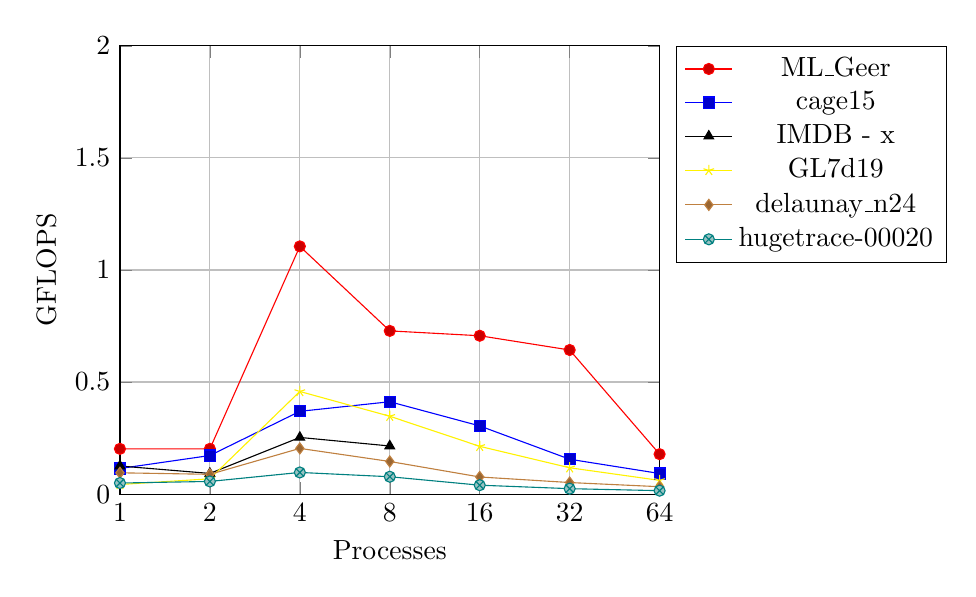
\begin{tikzpicture}
    \begin{axis}[
        xlabel={Processes},
        ylabel={GFLOPS},
        legend pos=outer north east, % Adjust the legend position
        grid=both, % Display grid lines
        xmode=log, % Set x-axis to logarithmic scale
        xmin=1, xmax=64, % Set x-axis limits
        ymin=0, ymax=2, % Set y-axis limits
        xtick={1,2,4,8,16,32,64}, % Specify the x-axis tick values
        xticklabels={1,2,4,8,16,32,64}, % Specify the labels for the tick values
        cycle multiindex list={
            color list\nextlist
            mark list
        }
      ]
      
      % Line 1
      \addplot coordinates {
        (1,0.202015)
        (2,0.202015)
        (4,1.10531)
        (8,0.72828)
        (16,0.706596)
        (32,0.64301)
        (64,0.178271)
        (128,0.145551)
      };
      \addlegendentry{ML\_Geer}
      
      % Line 2
      \addplot coordinates {
              (1,0.11429) 
              (2,0.172263)
              (4,0.369385) 
              (8,0.412145)
              (16,0.304342)
              (32,0.155641)
              (64,0.0920335)
      };
      \addlegendentry{cage15}
      
      % Line 3
      \addplot coordinates {
              (1,0.125482)
              (2, 0.0923397)
              (4,0.252987)
              (8,0.21477)
      };
      \addlegendentry{IMDB - x}
      \addplot coordinates {
              (1,0.0429374)
              (2, 0.0684547)
              (4,0.457955)
              (8,0.347466)
              (16,0.213221)
              (32,0.117609)
              (64,0.0613282)
      };
      \addlegendentry{GL7d19}
      \addplot coordinates {
              (1,0.0951383)
              (2, 0.0883726)
              (4,0.204037)
              (8,0.145655)
              (16,0.0765596)
              (32,0.0517325)
              (64,0.0331152)
      };
      \addlegendentry{delaunay\_n24}
      \addplot coordinates {
              (1,0.0494916)
              (2, 0.0566676)
              (4,0.0967503)
              (8,0.0775947)
              (16,0.0399043)
              (32,0.024393)
              (64,0.0154183)
      };
      \addlegendentry{hugetrace-00020}
      
      
    \end{axis}
  \end{tikzpicture}
  \caption{Defq - 1 Node}
\end{figure}
\end{frame}

\begin{frame}
\frametitle{Distributed Memory CSR - Total Execution Time}
\begin{figure}
  \centering
  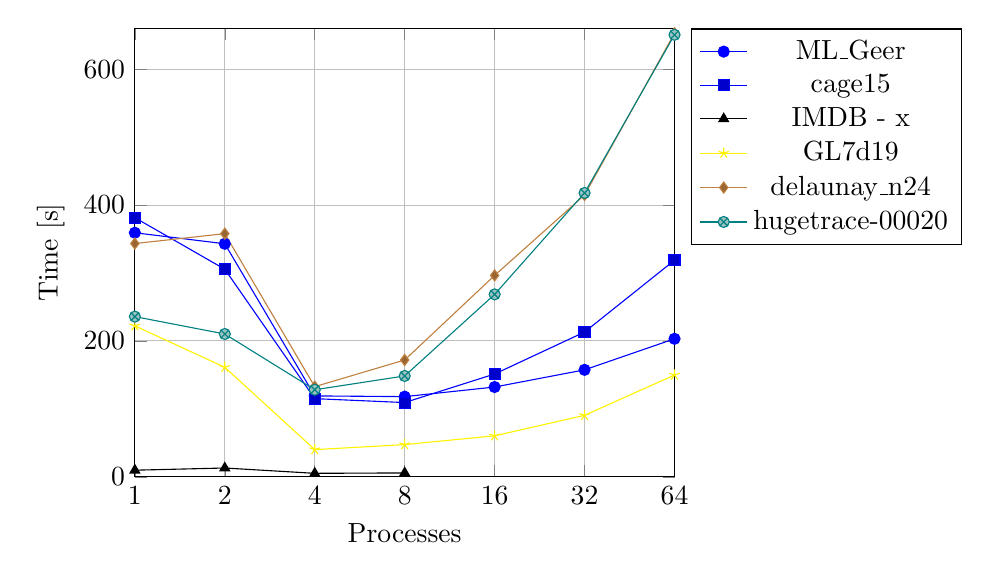
\begin{tikzpicture}
    \begin{axis}[
        xlabel={Processes},
        ylabel={Time [s]},
        legend pos=outer north east, % Adjust the legend position
        grid=both, % Display grid lines
        xmode=log, % Set x-axis to logarithmic scale
        xmin=1, xmax=64, % Set x-axis limits
        ymin=0, ymax=660, % Set y-axis limits
        xtick={1,2,4,8,16,32,64}, % Specify the x-axis tick values
        xticklabels={1,2,4,8,16,32,64}, % Specify the labels for the tick values
        cycle multiindex list={
            color list\nextlist
            mark list
        }
      ]
      
      % Line 1
      \addplot[blue, mark=*, mark options={blue}] coordinates {
        (1,359.253)
        (2,343.032)
        (4,119.062)
        (8,118.011)
        (16,132.142)
        (32,157.453)
        (64,203.149)
      };
      \addlegendentry{ML\_Geer}

      % Line 2
      \addplot coordinates {
              (1,381.482) 
              (2,305.591)
              (4,115.044) 
              (8,109.27)
              (16,151.302)
              (32,213.095)
              (64,318.84)
      };
      \addlegendentry{cage15}

      % Line 3
      \addplot coordinates {
              (1,9.71058)
              (2, 12.9307)
              (4,5.10052)
              (8,5.67675)
      };
      \addlegendentry{IMDB - x}
      \addplot coordinates {
              (1,222.229)
              (2, 161.219)
              (4,39.9891)
              (8,47.3685)
              (16,60.3243)
              (32,90.4711)
              (64,149.832)
      };
      \addlegendentry{GL7d19}
      \addplot coordinates {
              (1,343.366)
              (2, 357.939)
              (4,132.702)
              (8,171.949)
              (16,296.415)
              (32,414.84)
              (64,653.025)
      };
      \addlegendentry{delaunay\_n24}
      \addplot coordinates {
              (1,235.785)
              (2, 210.21)
              (4,128.117)
              (8,148.456)
              (16,268.53)
              (32,417.866)
              (64,650.659)
      };
      \addlegendentry{hugetrace-00020}
      
      
    \end{axis}
  \end{tikzpicture}
  \caption{Defq - 1 Node}
\end{figure}
\end{frame}

\begin{frame}
\frametitle{Distributed Memory CSR - Total Communication Time}
\begin{figure}
  \centering
  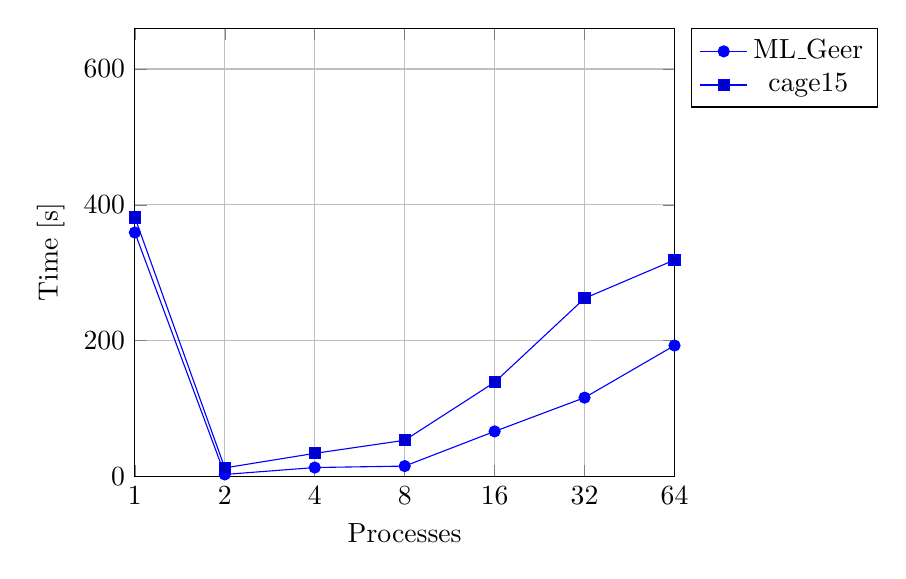
\begin{tikzpicture}
    \begin{axis}[
        xlabel={Processes},
        ylabel={Time [s]},
        legend pos=outer north east, % Adjust the legend position
        grid=both, % Display grid lines
        xmode=log, % Set x-axis to logarithmic scale
        xmin=1, xmax=64, % Set x-axis limits
        ymin=0, ymax=660, % Set y-axis limits
        xtick={1,2,4,8,16,32,64}, % Specify the x-axis tick values
        xticklabels={1,2,4,8,16,32,64}, % Specify the labels for the tick values
        cycle multiindex list={
            color list\nextlist
            mark list
        }
      ]
      
      % Line 1
      \addplot[blue, mark=*, mark options={blue}] coordinates {
        (1,359.253)
        (2,3.09405)
        (4,13.2506)
        (8,15.3937)
        (16,66.4605)
        (32,116.165)
        (64,192.912)
      };
      \addlegendentry{ML\_Geer}

      % Line 2
      \addplot coordinates {
              (1,381.482) 
              (2,12.7415)
              (4,34.1418) 
              (8,53.3642)
              (16,138.791)
              (32,262.35)
              (64,318.84)
      };
      \addlegendentry{cage15}

      % % Line 3
      % \addplot coordinates {
      %         (1,9.71058)
      %         (2, 12.9307)
      %         (4,5.10052)
      %         (8,5.67675)
      % };
      % \addlegendentry{IMDB - x}
      % \addplot coordinates {
      %         (1,222.229)
      %         (2, 161.219)
      %         (4,39.9891)
      %         (8,47.3685)
      %         (16,60.3243)
      %         (32,90.4711)
      %         (64,149.832)
      % };
      % \addlegendentry{GL7d19}
      % \addplot coordinates {
      %         (1,343.366)
      %         (2, 357.939)
      %         (4,132.702)
      %         (8,171.949)
      %         (16,296.415)
      %         (32,414.84)
      %         (64,653.025)
      % };
      % \addlegendentry{delaunay\_n24}
      % \addplot coordinates {
      %         (1,235.785)
      %         (2, 210.21)
      %         (4,128.117)
      %         (8,148.456)
      %         (16,268.53)
      %         (32,417.866)
      %         (64,650.659)
      % };
      % \addlegendentry{hugetrace-00020}
      
      
    \end{axis}
  \end{tikzpicture}
  \caption{Defq - 1 Node}
\end{figure}
\end{frame}

\begin{frame}
\frametitle{Total time - Task A and Sequential}
\begin{figure}
  \centering
  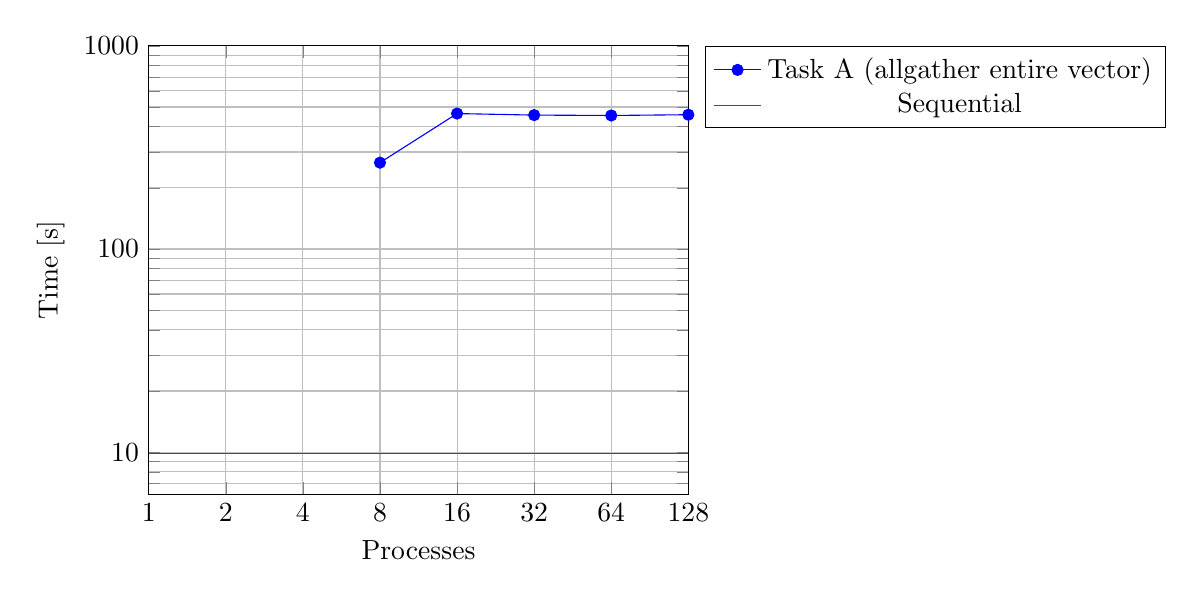
\begin{tikzpicture}
    \begin{axis}[
        xlabel={Processes},
        ylabel={Time [s]},
        legend pos=outer north east, % Adjust the legend position
        grid=both, % Display grid lines
        xmode=log, % Set x-axis to logarithmic scale
        ymode=log,
        xmin=1, xmax=128, % Set x-axis limits
        ymin=0, ymax=1000, % Set y-axis limits
        xtick={1,2,4,8,16,32,64,128}, % Specify the x-axis tick values
        ytick={0.1,0.2,0.3,0.4,0.5,0.6,0.7,0.8,0.9,1,2,3,4,5,6,7,8,9,10,20,30,40,50,60,70,80,90,100,200,300,400,500,600,700,800,900,1000}, 
        yticklabels={0.1,\phantom{a},\phantom{a},\phantom{a},\phantom{a},\phantom{a},\phantom{a},\phantom{a},\phantom{a},1,\phantom{a},\phantom{a},\phantom{a},\phantom{a},\phantom{a},\phantom{a},\phantom{a},\phantom{a},10,\phantom{a},\phantom{a},\phantom{a},\phantom{a},\phantom{a},\phantom{a},\phantom{a},\phantom{a},100,\phantom{a},\phantom{a},\phantom{a},\phantom{a},\phantom{a},\phantom{a},\phantom{a},\phantom{a},1000}, 
        xticklabels={1,2,4,8,16,32,64,128}, % Specify the labels for the tick values
      ]
      
      % Line 1
      \addplot[blue, mark=*, mark options={blue}] coordinates {
              (8,266)
              (16,464)
              (32,456)
              (64,454)
              (128,458)
      };
      \addlegendentry{Task A (allgather entire vector)}
      \addplot[red] coordinates {
              (1,9.86)
              (128,9.86)
      };
      \addlegendentry{Sequential}
     
     
    \end{axis}
  \end{tikzpicture}
  \caption{Total time - scale 12}
\end{figure}

\end{frame}

\begin{frame}
\frametitle{Results of Row, Column and Grid based multiplication}
\begin{figure}
  \centering
  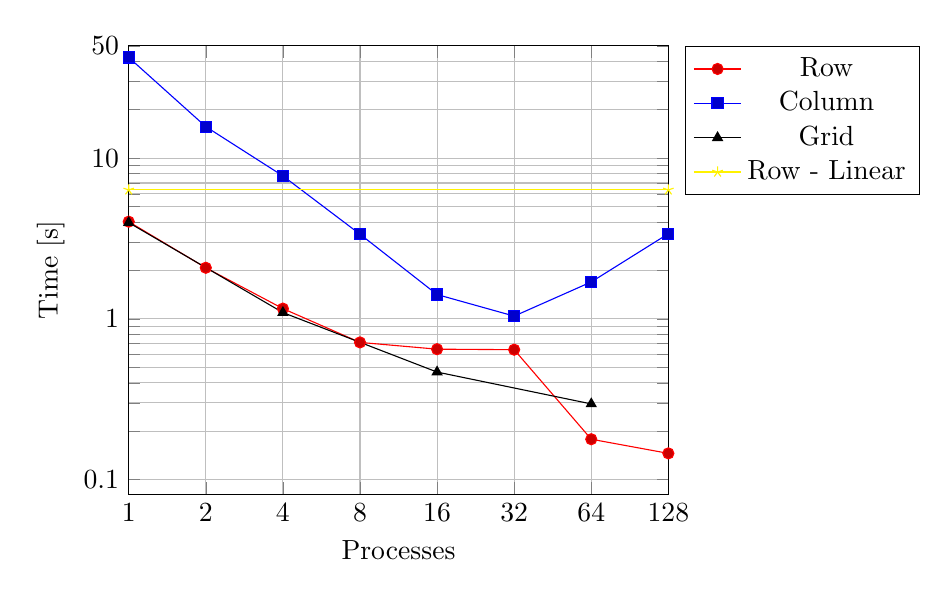
\begin{tikzpicture}
    \begin{axis}[
        xlabel={Processes},
        ylabel={Time [s]},
        legend pos=outer north east, % Adjust the legend position
        grid=both, % Display grid lines
        xmode=log, % Set x-axis to logarithmic scale
        ymode=log,
        xmin=1, xmax=128, % Set x-axis limits
        ymin=0, ymax=50, % Set y-axis limits
        xtick={1,2,4,8,16,32,64,128}, % Specify the x-axis tick values
        ytick={0.1,0.2,0.3,0.4,0.5,0.6,0.7,0.8,0.9,1,2,3,4,5,6,7,8,9,10,20,30,40,50}, % Specify the y-axis tick values you want to label
        yticklabels={0.1,\phantom{a},\phantom{a},\phantom{a},\phantom{a},\phantom{a},\phantom{a},\phantom{a},\phantom{a},1,\phantom{a},\phantom{a},\phantom{a},\phantom{a},\phantom{a},\phantom{a},\phantom{a},\phantom{a},10,\phantom{a},\phantom{a},\phantom{a},50}, % Specify the labels for the y-axis tick values you want to label
        xticklabels={1,2,4,8,16,32,64,128}, % Specify the labels for the tick values
        cycle multiindex list={
            color list\nextlist
            mark list
        }
      ]

      
      % Line 1
      \addplot coordinates {
        (1,4.02475)
        (2,2.07932)
        (4,1.15842)
        (8,0.713717)
        (16,0.647709)
        (32,0.64301)
        (64,0.178271)
        (128,0.145551)
      };
      \addlegendentry{Row}
      
      % Line 2
      \addplot coordinates {
              (1,42.3427) 
              (2,15.7043)
              (4,7.75336) 
              (8,3.36393)
              (16,1.41673)
              (32,1.04024)
              (64,1.69703)
              (128,3.3874)
      };
      \addlegendentry{Column}
      
      % Line 3
      \addplot coordinates {
              (1,3.97187)
              (4,1.09431)
              (16,0.466605)
              (64,0.295661)
      };
      \addlegendentry{Grid}
      \addplot coordinates {
        (1,6.34598)
        (128,6.34598)
      };
      \addlegendentry{Row - Linear}
      
      
    \end{axis}
  \end{tikzpicture}
  \caption{Total time - scale 15}
\end{figure}
\end{frame}

\end{document}
